
\textbf{\textit{Positional Encoding}}. In order for the model to make use of the order of the sequence, we need to inject somne information about the position of the frames. For simplicity, we add an additional embedding layer to embed the relative position of the frame. Specifically, the embedded position index is concatenated with the hidden features before the final segmentation head. The relative position of $k^{th}$ frame of CT volume $i$ with length $T_i$ is calculated as:

\begin{align}
        PE(k) &= \frac{k}{T_i}
\end{align}

We attach this layer to both DeeplabV3+ and TransUnet. Since they follows conventional structure of segmentation models, which comprise of encoder and decoder phases, we manage to attach the layer in a similar way for both of them, as can be generally seen in Figure \ref{fig:pe_arch}

\begin{figure}[!h]
    \centering
    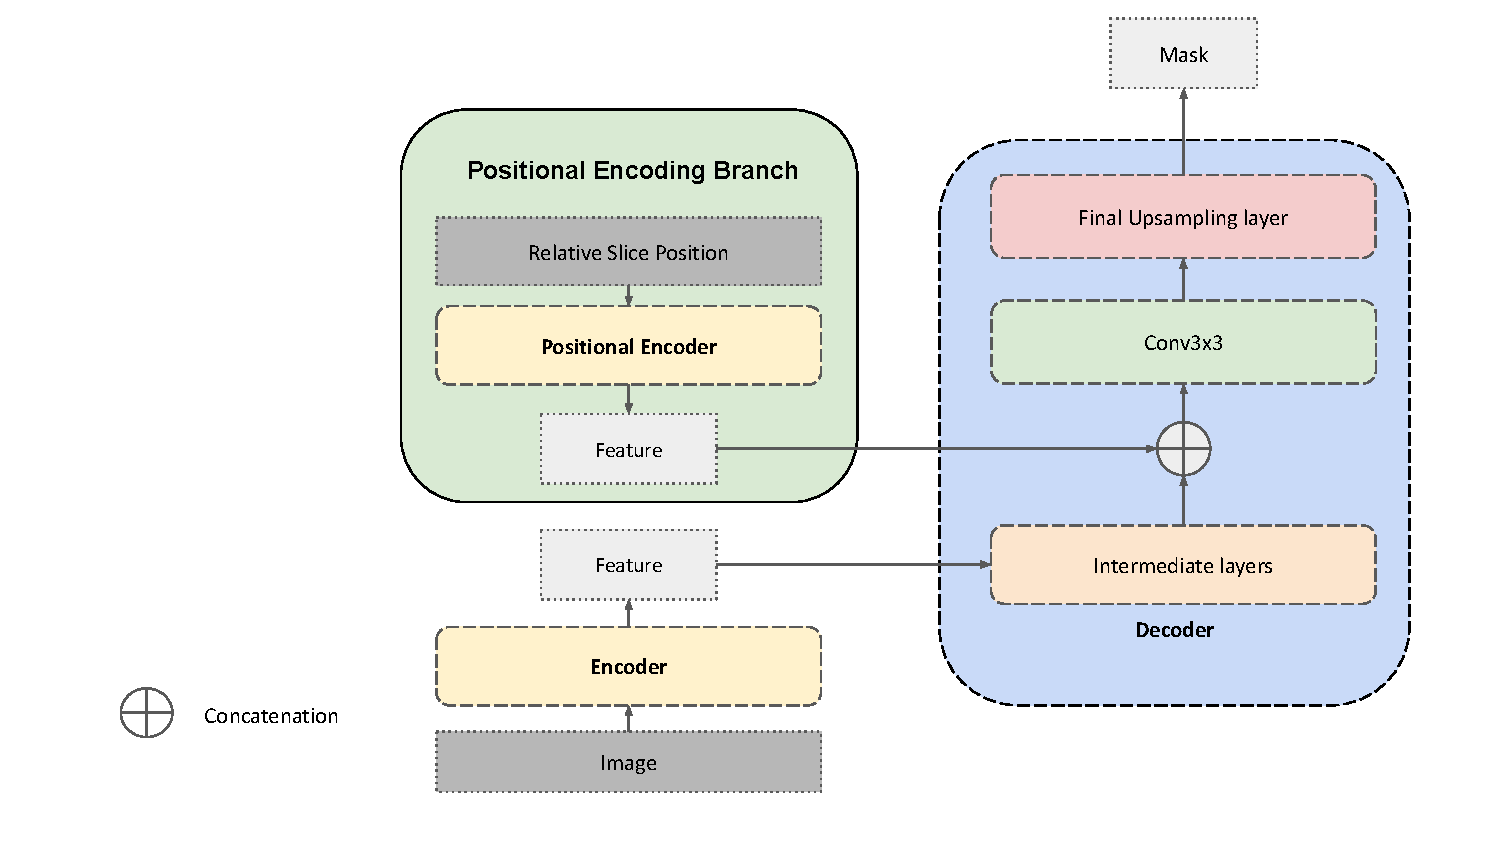
\includegraphics[width=\textwidth]{resources/new_images/pe.pdf}
    \caption{A general and simple way to attach a Positional Encoding branch into segmentation models . }
    \label{fig:pe_arch}
\end{figure}